\documentclass{article}
\usepackage[utf8]{inputenc}
\usepackage{graphicx}

\title{TUGAS PEMROGRAMAN 2}
\author{Dian Markuci (1184095) }
\date{17 Oktober 2019}

\begin{document}

\maketitle
\begin{center}

    
\end{center}

\section{Sejarah Python}
\usepackage{Pertama kali python diciptakan di Centrum Wiskunde & Informatica (CWI), Belanda pada awal tahun 1990-an. Penciptanya adalah Guido Van Rassum yang terinspirasi dari bahasa pemrograman ABC. Sampai saat ini Guido masih menjadi penulis utama untuk python. Python bersifat open source sehingga ribuan orangpun ikut berkontribusi dalam pengembangannya. Pada tahun 1995, Guido melanjutkan pembuatan python di CNRI di Virginia Amerika, dimana Guido menulis beberapa versi python.Pada tahun 2001, organisasi python di bentuk namanya adalah Python Software Foundation(PSF). PSF sendiri adalah organisasi nirlaba yang dibuat secara khusus untuk segala hal yang berkaitan dengan hak intelektual Python. Nama python tidak berasal dari nama ular. Guido adalah penggemar grup komedi Inggris bernama Monty Python. lalu kemudian ia memberi nama bahasa ciptaannya"Python".}

\section{Perbedaan Python 2 dan 3}
\usepackage{Ada dua versi python yang popular saat ini, yaitu python versi 2 dan python versi 3, lalu apakah perbedaannya? simak penjelasan di bawah ini}
\subsection{Python 2}
\usepackage{Dipublikasi pada sekitar akhir tahun 2000,Penilaian mengenai Python 2 yaitu lebih inklusif dan transparan untuk perkembangan software dibandingkan versi sebelumnya. Hal tersebut didukung adanya PEP – Python Enhancement Proposal, yaitu sebuah spesifikasi teknis yang menjadi tuntunan informasi untuk user dan penggambaran fitur baru pada Python tersebut. Python 2 juga dilengkapi berbagai fitur programatikal seperti cycle-detecting garbage collector sebagai  peningkatan dukungan untuk Unicode,otomasi manajemen memori, list comprehension untuk membuat sebuah list berdasar list yang telah ada. Unifikasi pada tipe data Python dan class ke satu hirarki terjadi pada rilis Python 2.2}

\subsection{Python 3}
\usepackage{Python 3 merupakan pengembangan dari python versi 2 sebagai harapan masa depan Python. Python 3 merupakan versi dengan perubahan yang banyak dan telah dirilis pada akhir tahun 2008. Fokus Python 3 itu yaitu merapikan codebase dan menghapuskan duplikasi atau redundancy. Termasuk memasukkan statemen print ke dalam built-in function merupakan perubahan terbesar python 3.Awalnya, pada pengadopsian Python 3 mengalami hambatan dikarenakan akibat dari tidak adanya backwards compatibility dengan Python 2. Hal ini mengakibatkan pengguna Python sangat berat hati karena harus pindah ke versi 3. Untuk Tambahan, banyak library yang tersedia hanya untuk Python 2., namun semakin banyak libary disalin ke Python 3, penerapan Python 3 maka semakin lama akan semakin meningkat.}

\section{Implementasi dan Penggunaan Python di Perusahaan Dunia}
\usepackage{Python adalah bahasa pemrograman yang populer dan cocok untuk di pelajari. Penasaran ga sih siapa aja yang gunaik python? Simak ya uraian dibawah ini: Google,Youtube,Facebook,Instagram,Pinterest,Dropbox,Quora,NASA, NSA,Industrial Light & Magic, Pixar,Blender, Maya, software pembuat animasi 3D,Raspberry Pi,ESRI,dan masih banyak lain}
\subsection{Implementasi}
\usepackage{Untuk kali ini saya mengambil contoh beberapa platform yang menggunakan python dalam analisis data, platform terbaru dan terpopuler saat ini yaitu spotify dan netflix. Dalam penerapannya kedua platform ini, utamanya terlihat pada bagaimana Spotify merekomendasikan lagu dan Netflix merekomendasikan film kepada para pelanggannya. berikut merupakan poin-poin tentang implementasi python dalam analisis data spotify:}
\begin{enumerate}
    \item Pemanfaatan analitis oleh Tim Spotify.dengan modul dari python mereka memanfaatkan Luigi yang di sinkronisasi dengan Hadoop yaitu sebuah framework basis java untuk digunakan sebagai pemrosesan data dengan ukuran yang sangat besar.
    \item Luigi dimanfaatkan untuk kemungkinan membangun pipeline kompleks secara cepat. dan mampu menangani bundling library yang dibutuhkan, serta dapat mengembalikan error log ke komputer lokal.
    \item Selain itu Spotify mengaplikasikan Luigi dengan berbagai algoritme machine learning untuk menghidupkan fitur Radio dan Discover, serta rekomendasi untuk orang yang mungkin ingin diikuti.
    \item Pada laman Spotify Labs, Spotify juga menyatakan bahwa mereka menggunakan bahasa pemrograman Python dalam sembilan puluh persen urusan MapReduce mereka. Data Science Graduate Program mengibaratkan Hadoop sebagai sumber hidup big data, sementara MapReduce berperan sebagai detak jantungnya.
\end{enumerate}

\section{Instalasi}
\graphicspath{{gambar/anaconda}}
\subsection{Instalasi anaconda}
\paragraph{}
\begin{itemize}
	\item Langkah awal kunjungi dulu website anaconda (https://www.anaconda.com/distribution/\#download-section), download python sesuai dengan sistem operasi yang dipakai\\
	\begin{center}
	    	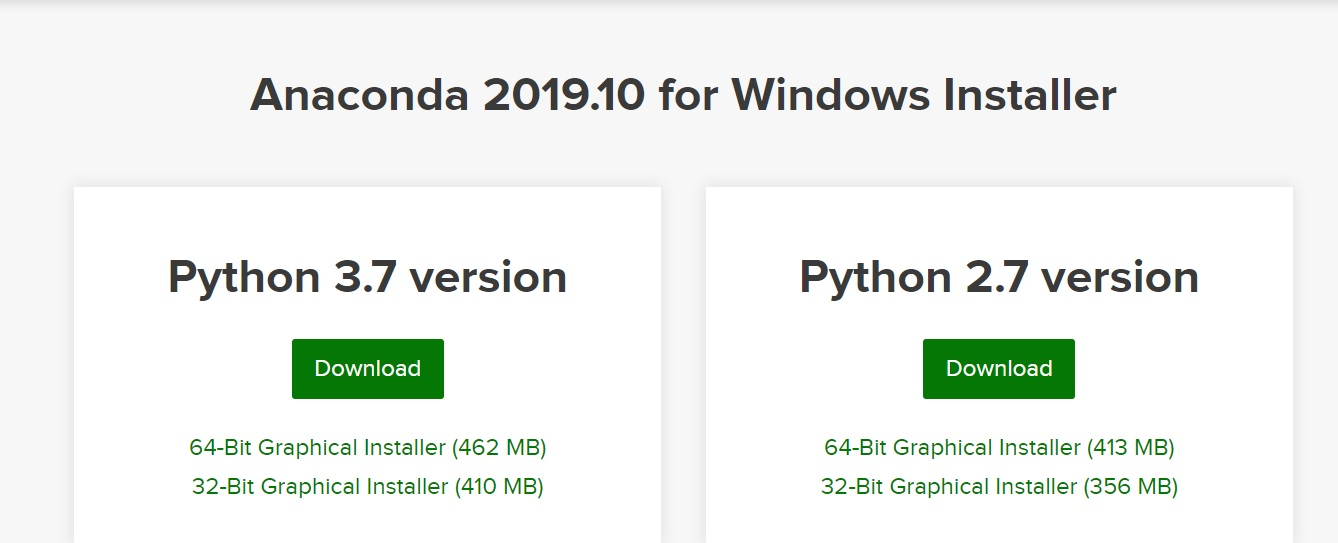
\includegraphics[width=7.5cm]{SS A1.jpg} 
	\end{center}

	\item Buka file installer, Klik "next"\\
	
	\item Klik "I agree"\\
	
	\item Klik "next"\\

	\item Tentukan lokasi folder anaconda yang akan di install lalu klik "next"\\
	
	\item Klik cetang pada "Add anaconda to my PATH environment variable" lalu klik "next"\\

	\item Tunggu hingga proses selesai lalu klik "next"\\

	\item Klik "next"\\
	
	\item Klik "finish"\\

\end{itemize}
\subsection{Instalasi Python}
\paragraph{}
\begin{itemize}
	\item Langkah awal kunjungi dulu website python, download sesuai pilihan user, rekomendasi versi 3 
	\item Pilih install now, tapi jangan lupa tambahan centang untuk add path\\
	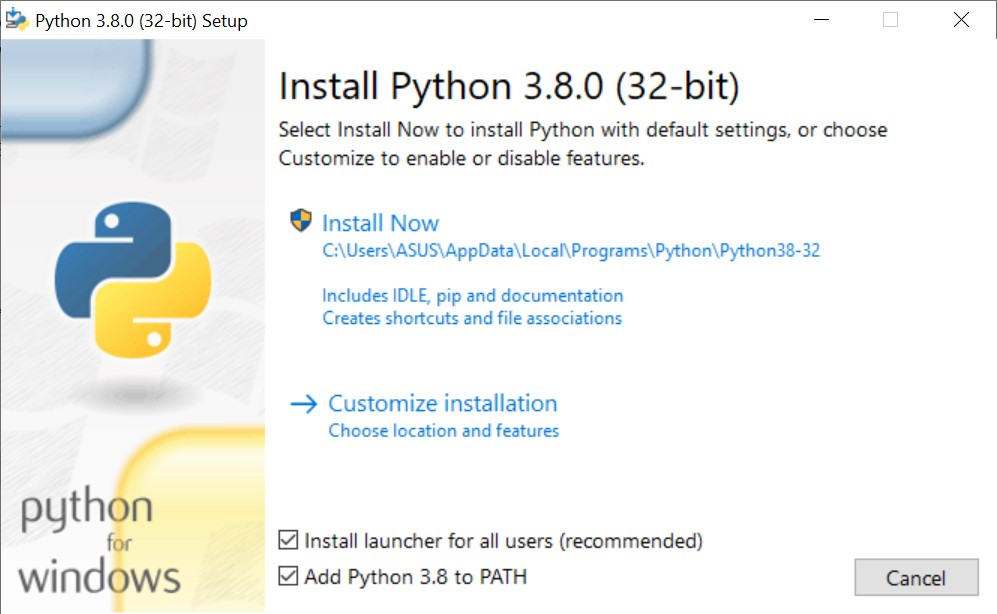
\includegraphics[width = 10cm]{python1.jpg}\\ 
	\item Tunggu\\
	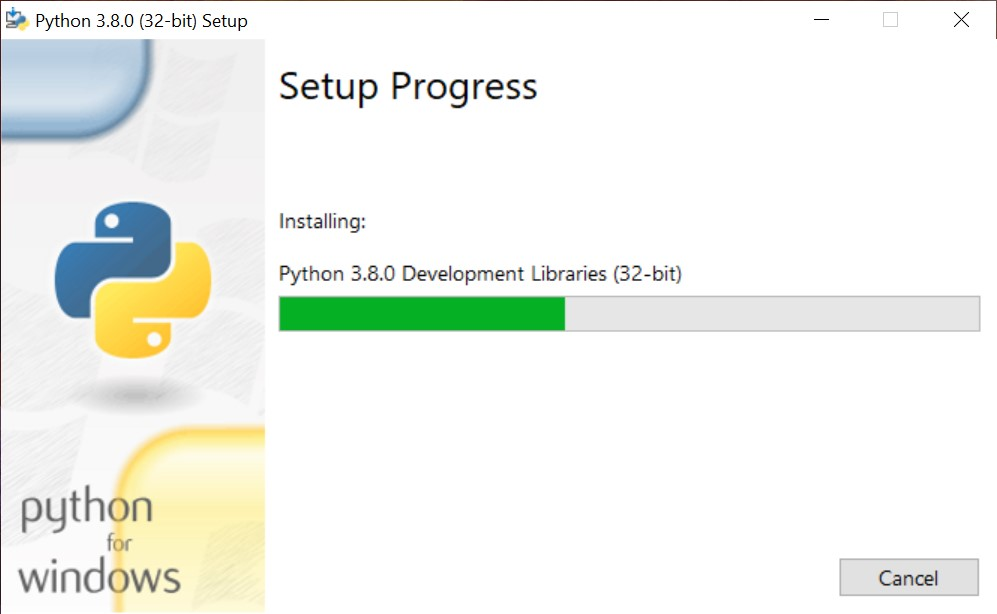
\includegraphics[width = 10cm]{tunggu.jpg}\\ 
	\item Sukses\\
	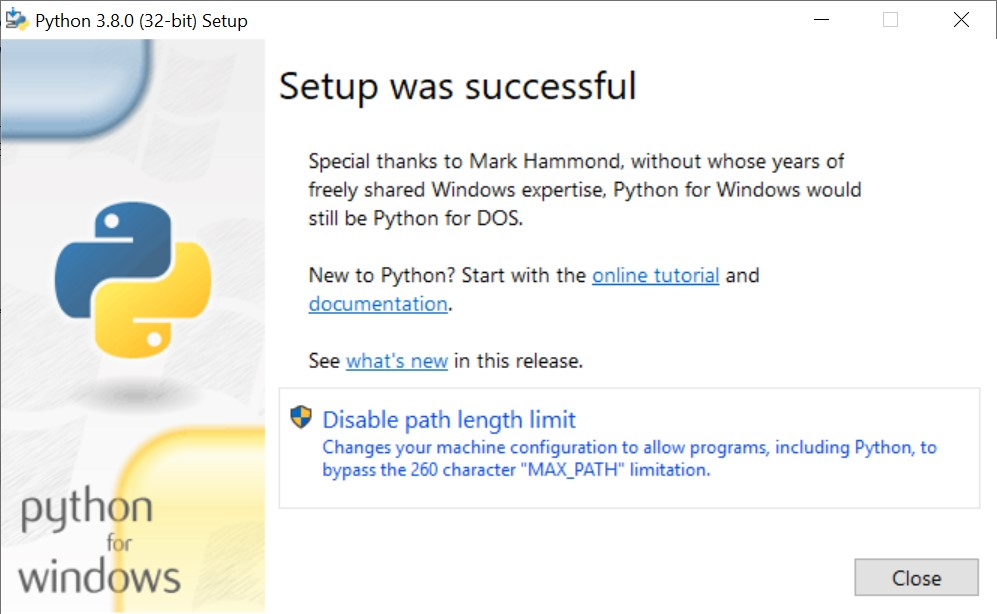
\includegraphics[width = 10cm]{sukses.jpg}\\

\end{itemize}

\subsection{Instalasi Pip}
\paragraph{},
\begin{itemize}
    \item Ketikan Pip di CMD
    \begin{center}
        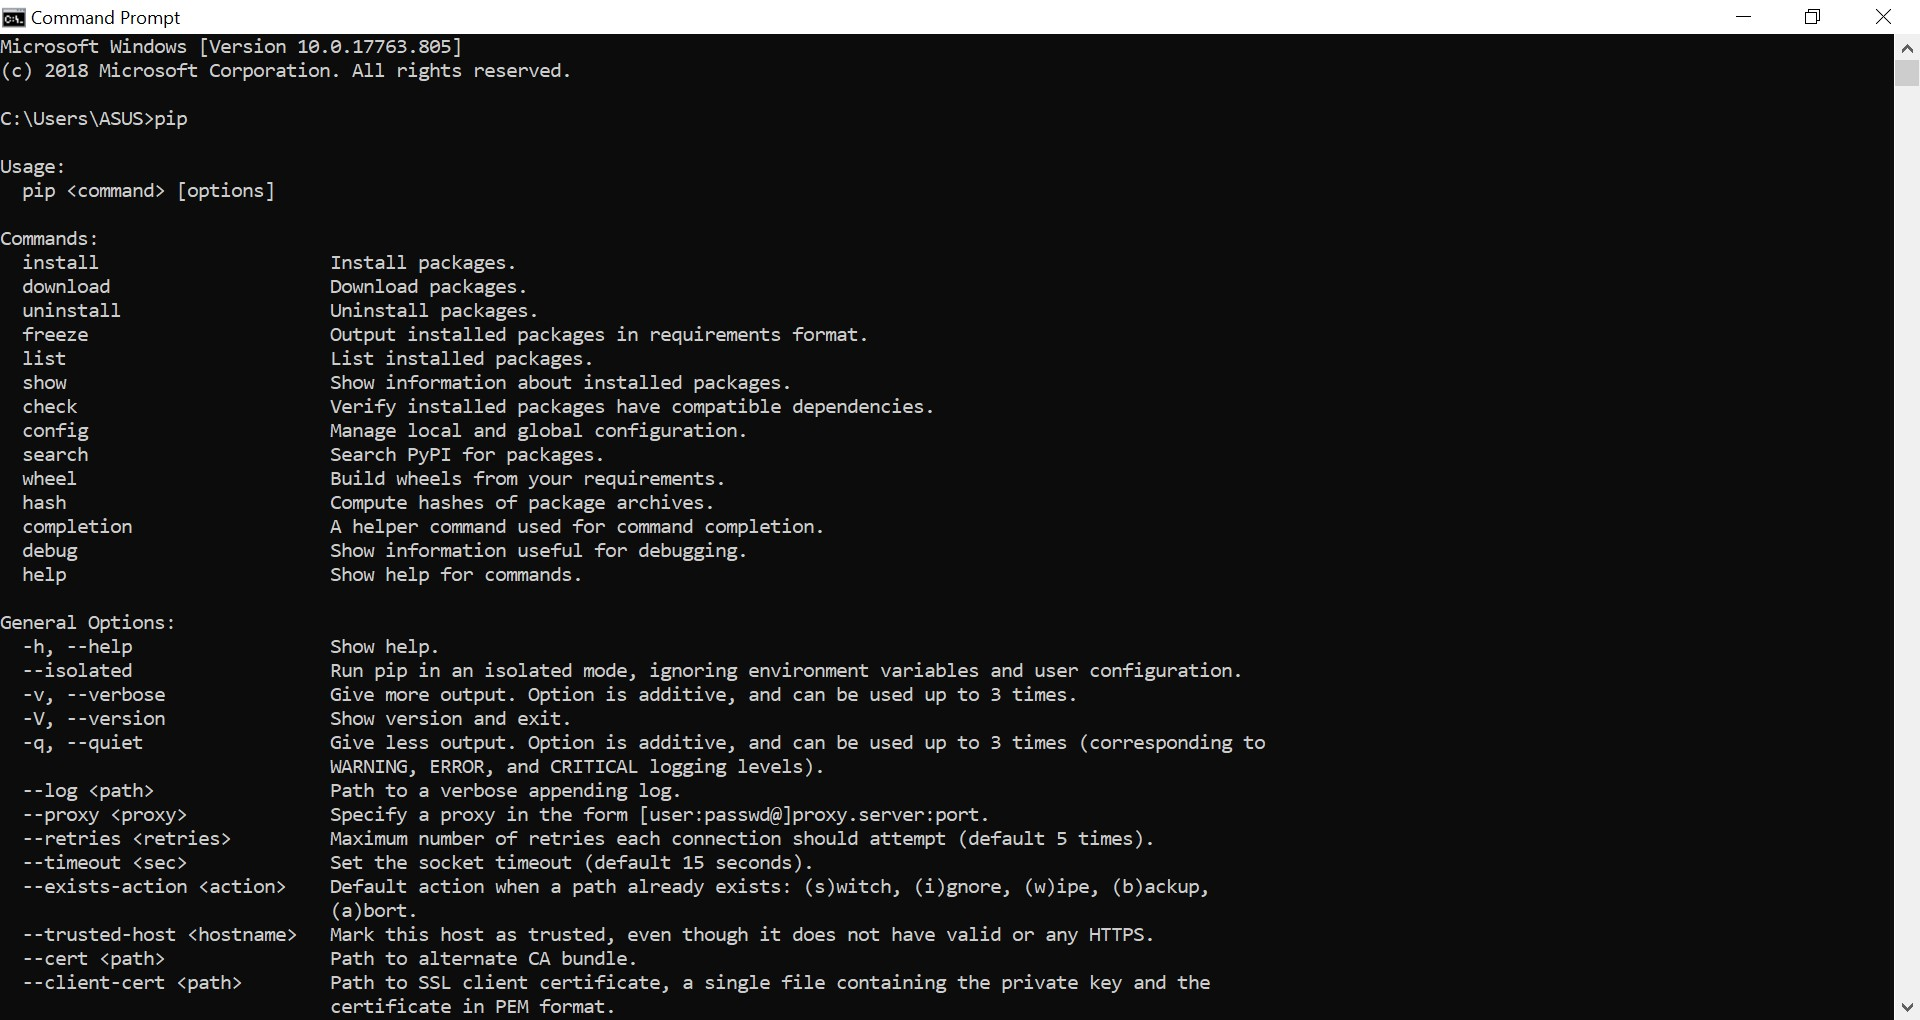
\includegraphics[width = 10cm]{pip.jpg}
    \end{center}
    
\end{itemize}

\subsection{Setting Environment}
\paragraph{}
\begin{itemize}
    \item Buka CMD, ketikan "python" apabila dikenali maka tidak perlu setting environment variable, begini tampilannya:
    \begin{center}
        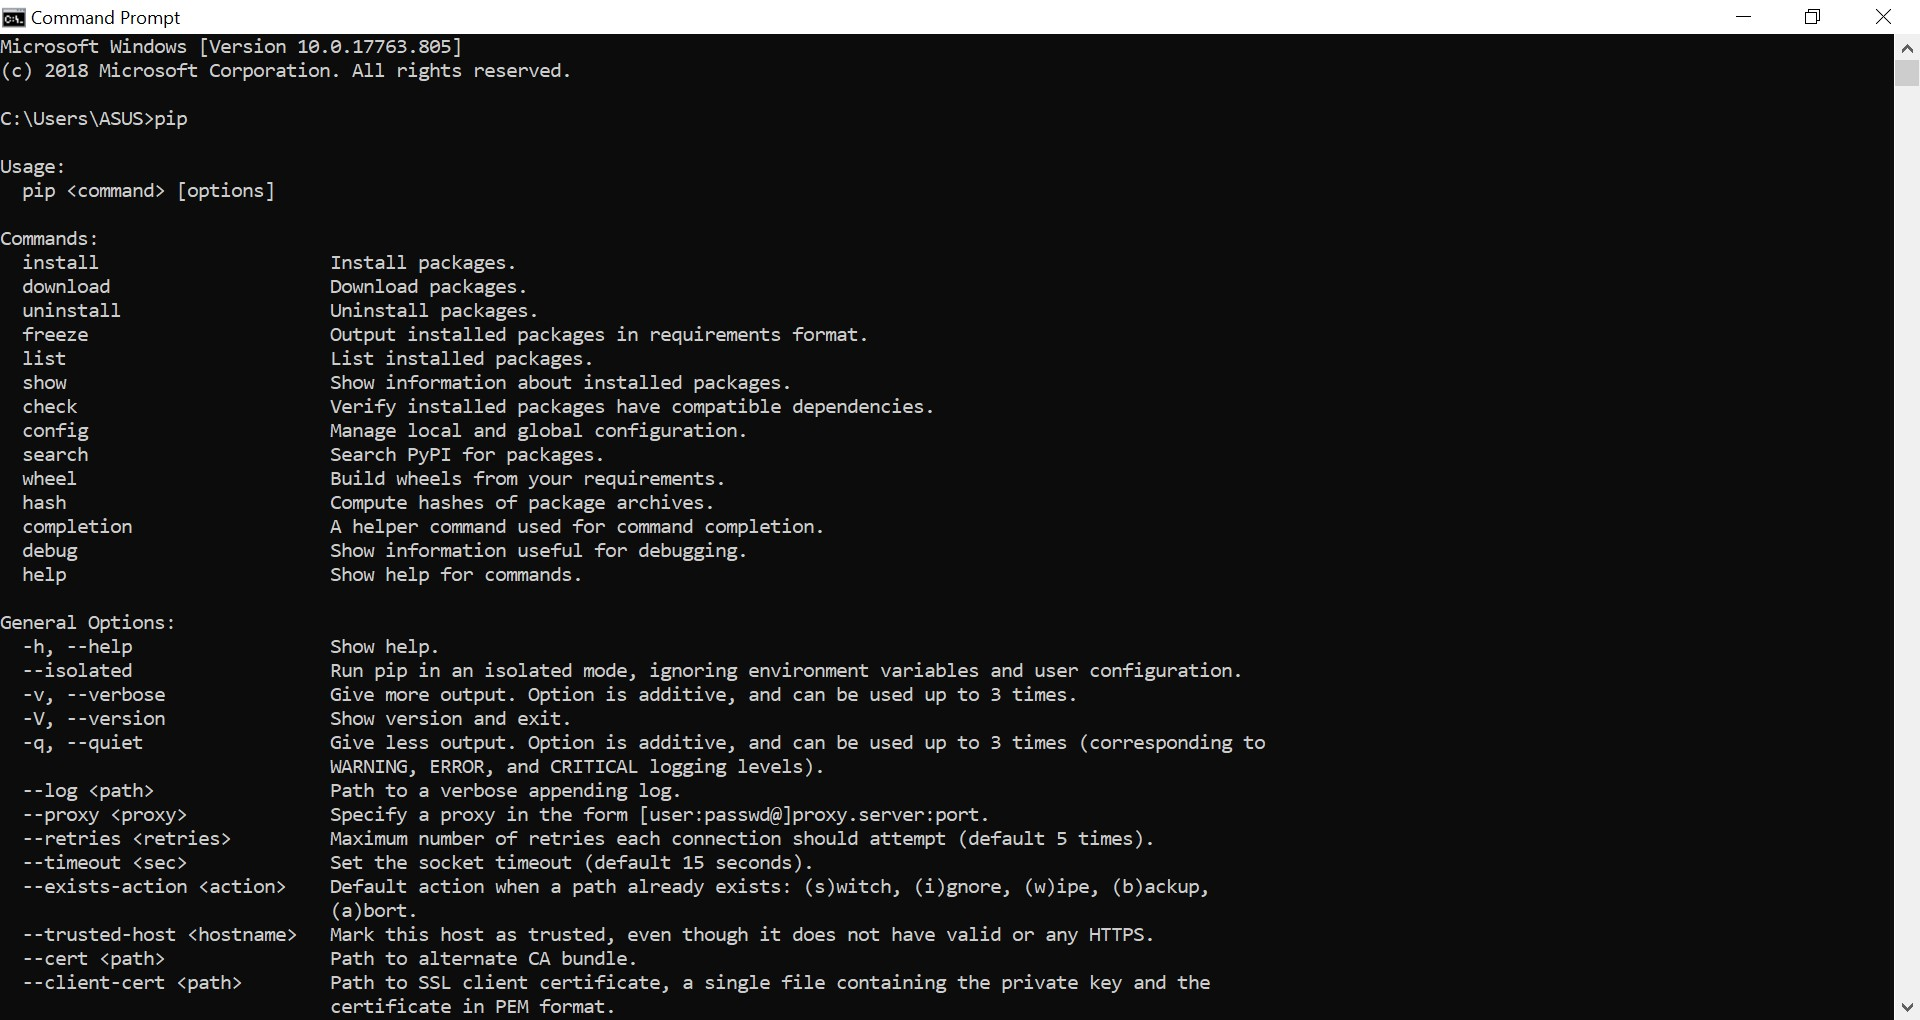
\includegraphics[width = 10cm]{pip.jpg}
    \end{center}
    
\end{itemize}

\subsection{ mencoba entrepreter/cli di cmd windows}
\paragraph{}
\begin{itemize}
    \item Pertama, kita coba dulu membuka Python Shell. Silahkan masuk ke manu kemudian cari Python Shell.\\
    \item dari CMD, ketik perintah python untuk masuk ke Python Shell dari CMD,\\
    \item Ketikkan perintah di IDLE dan Hasilnya maka:
    \begin{center}
        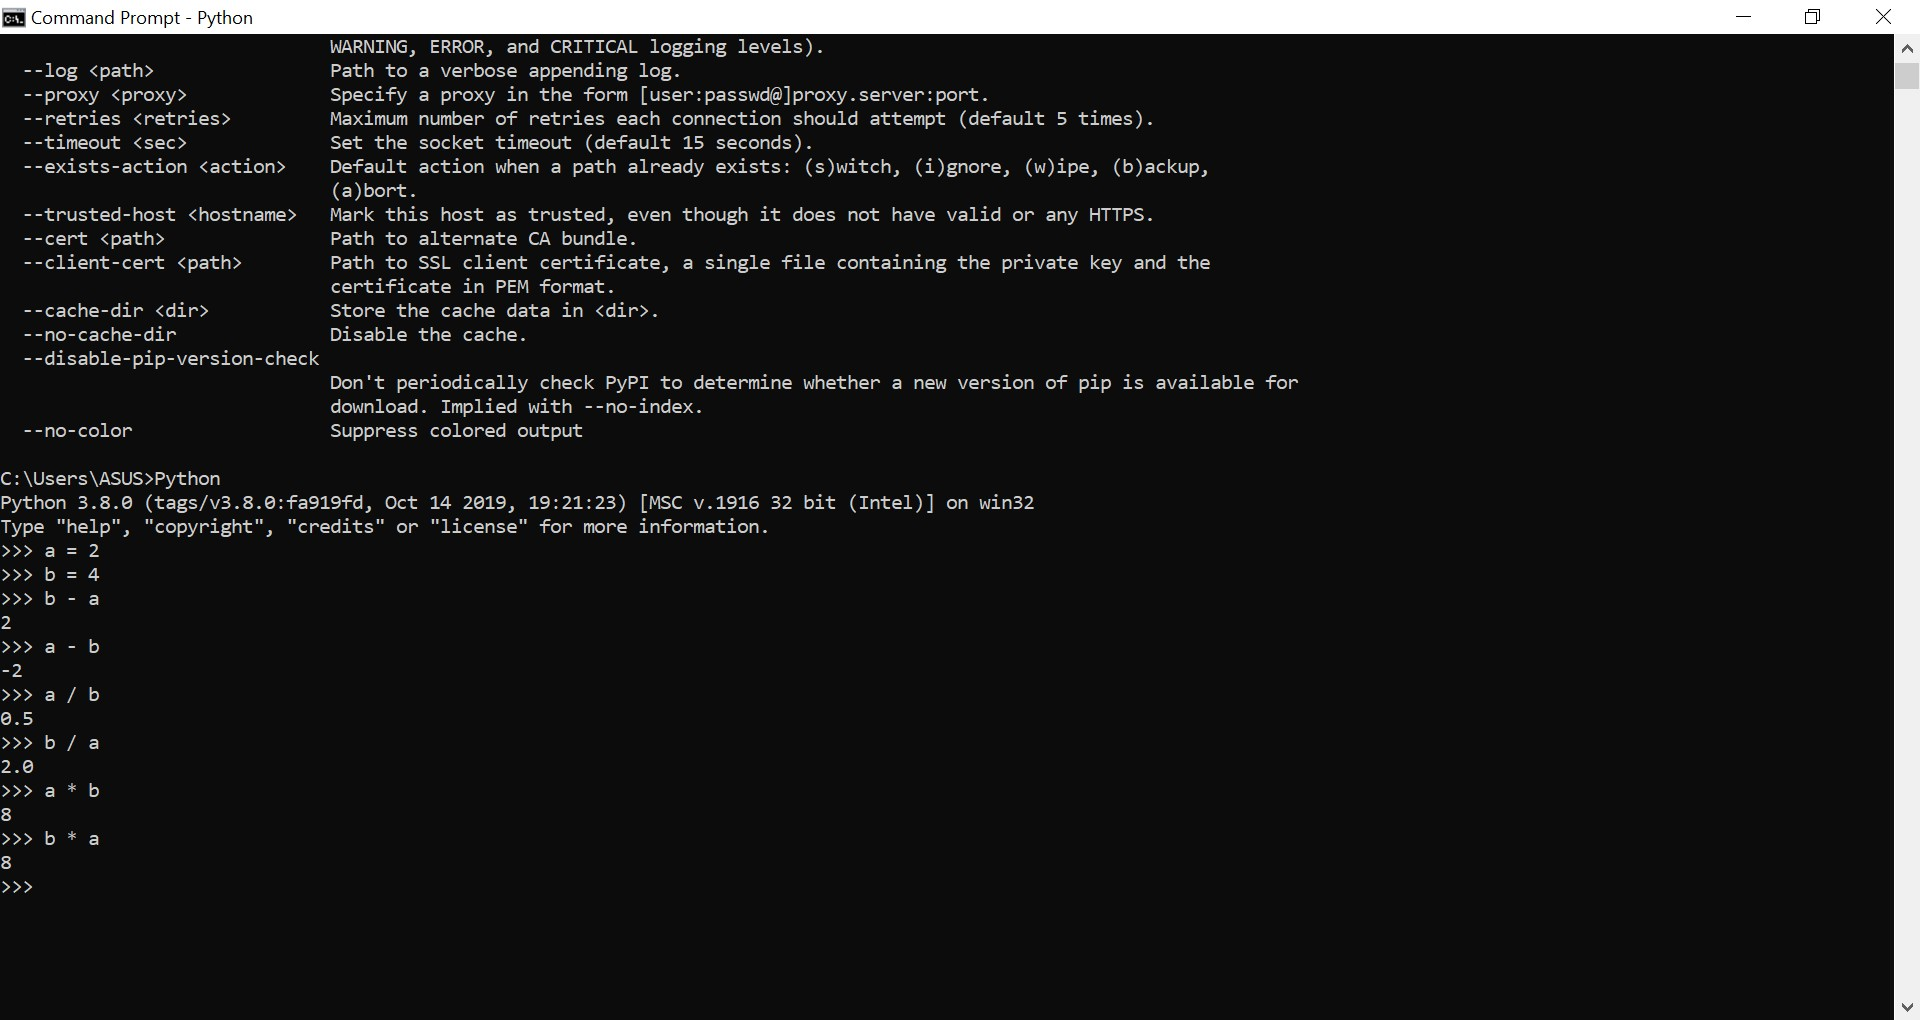
\includegraphics[width = 10cm]{preter.jpg}
    \end{center}
\end{itemize}

\subsection{Print hello world}
\paragraph{}
\begin{itemize}
	\item Buka spyder\\
	\item tuliskan syntax print("hello world")
	\item klik run script atau tekan F5
	\begin{center}
	    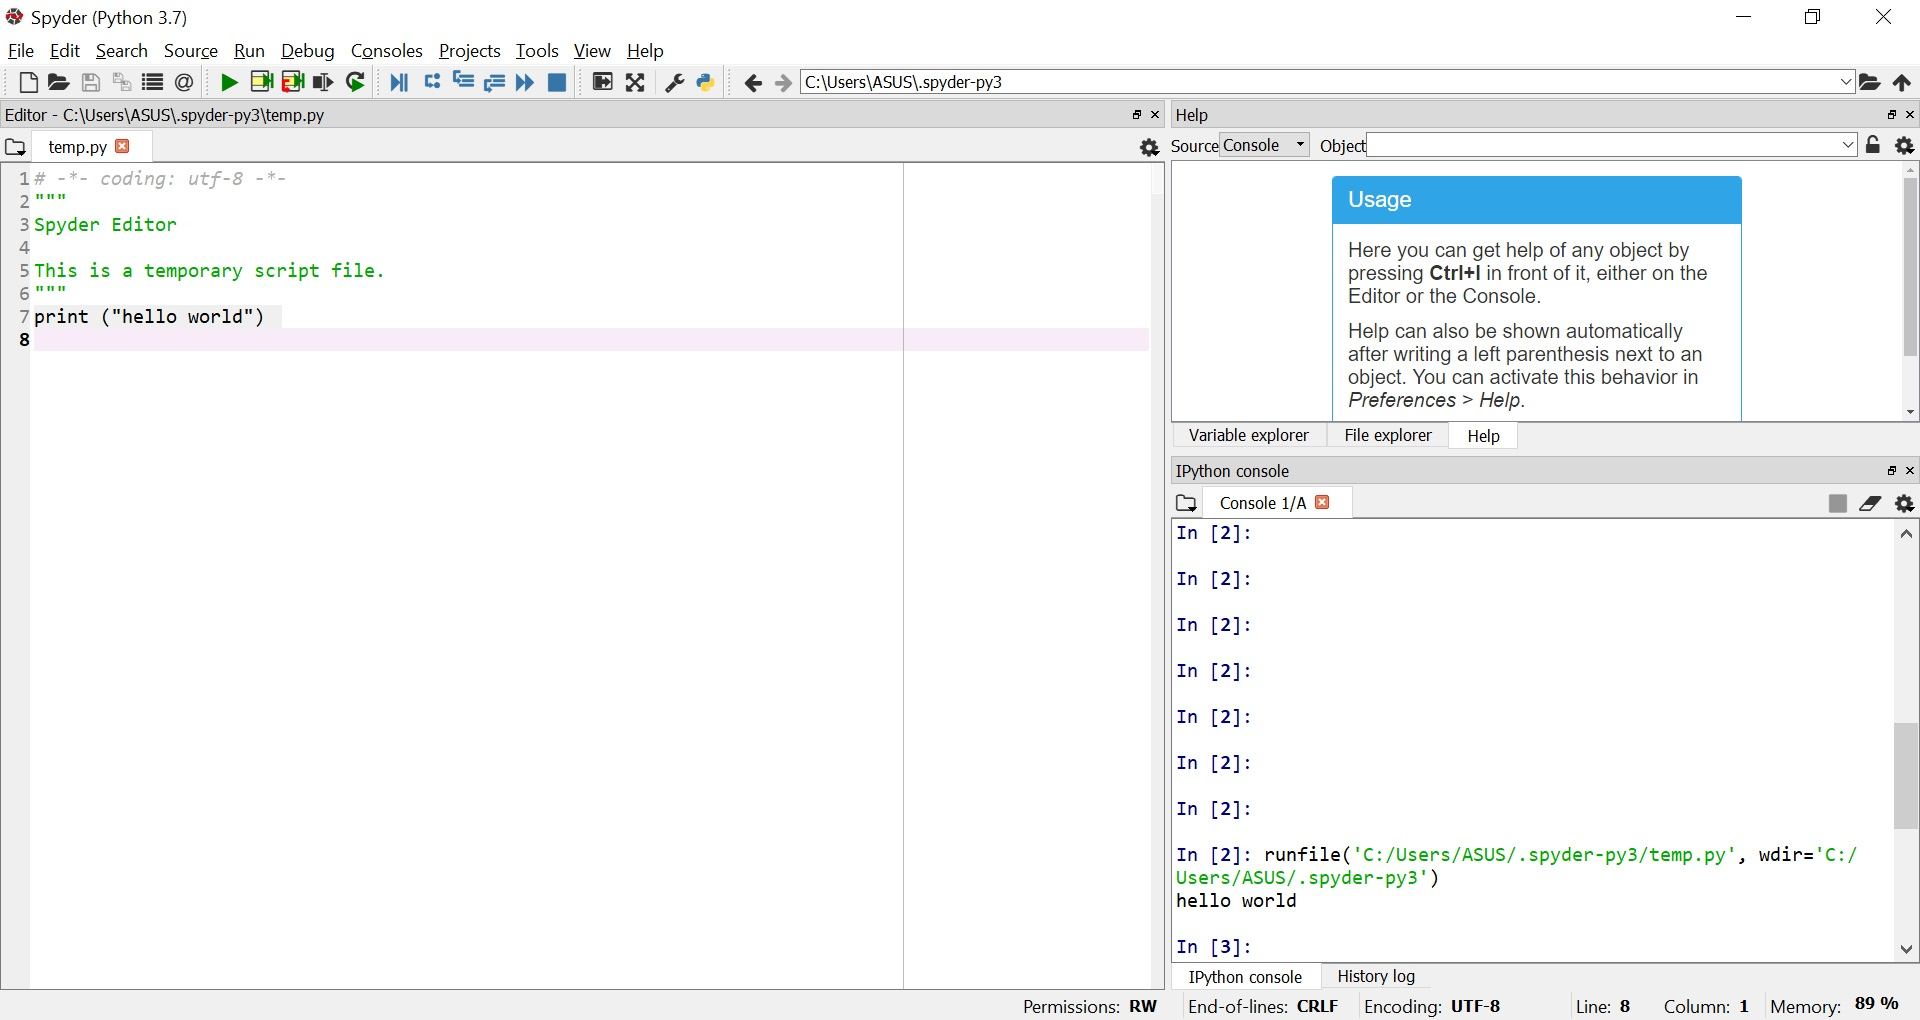
\includegraphics[width = 10cm]{hello.jpg}
	\end{center}
	\item tuliskan nama file lalu klik save\\

\end{itemize}

\subsection{Variable exploler}
\paragraph{}
Variabel exploler digunakan sebagai pengecekan semua variabel yang punya value\\

\subsection{ Cara menjalankan Script otomatis login aplikasi akademik dengan library selenium dan inputan user}
\paragraph{}
\begin{center}
    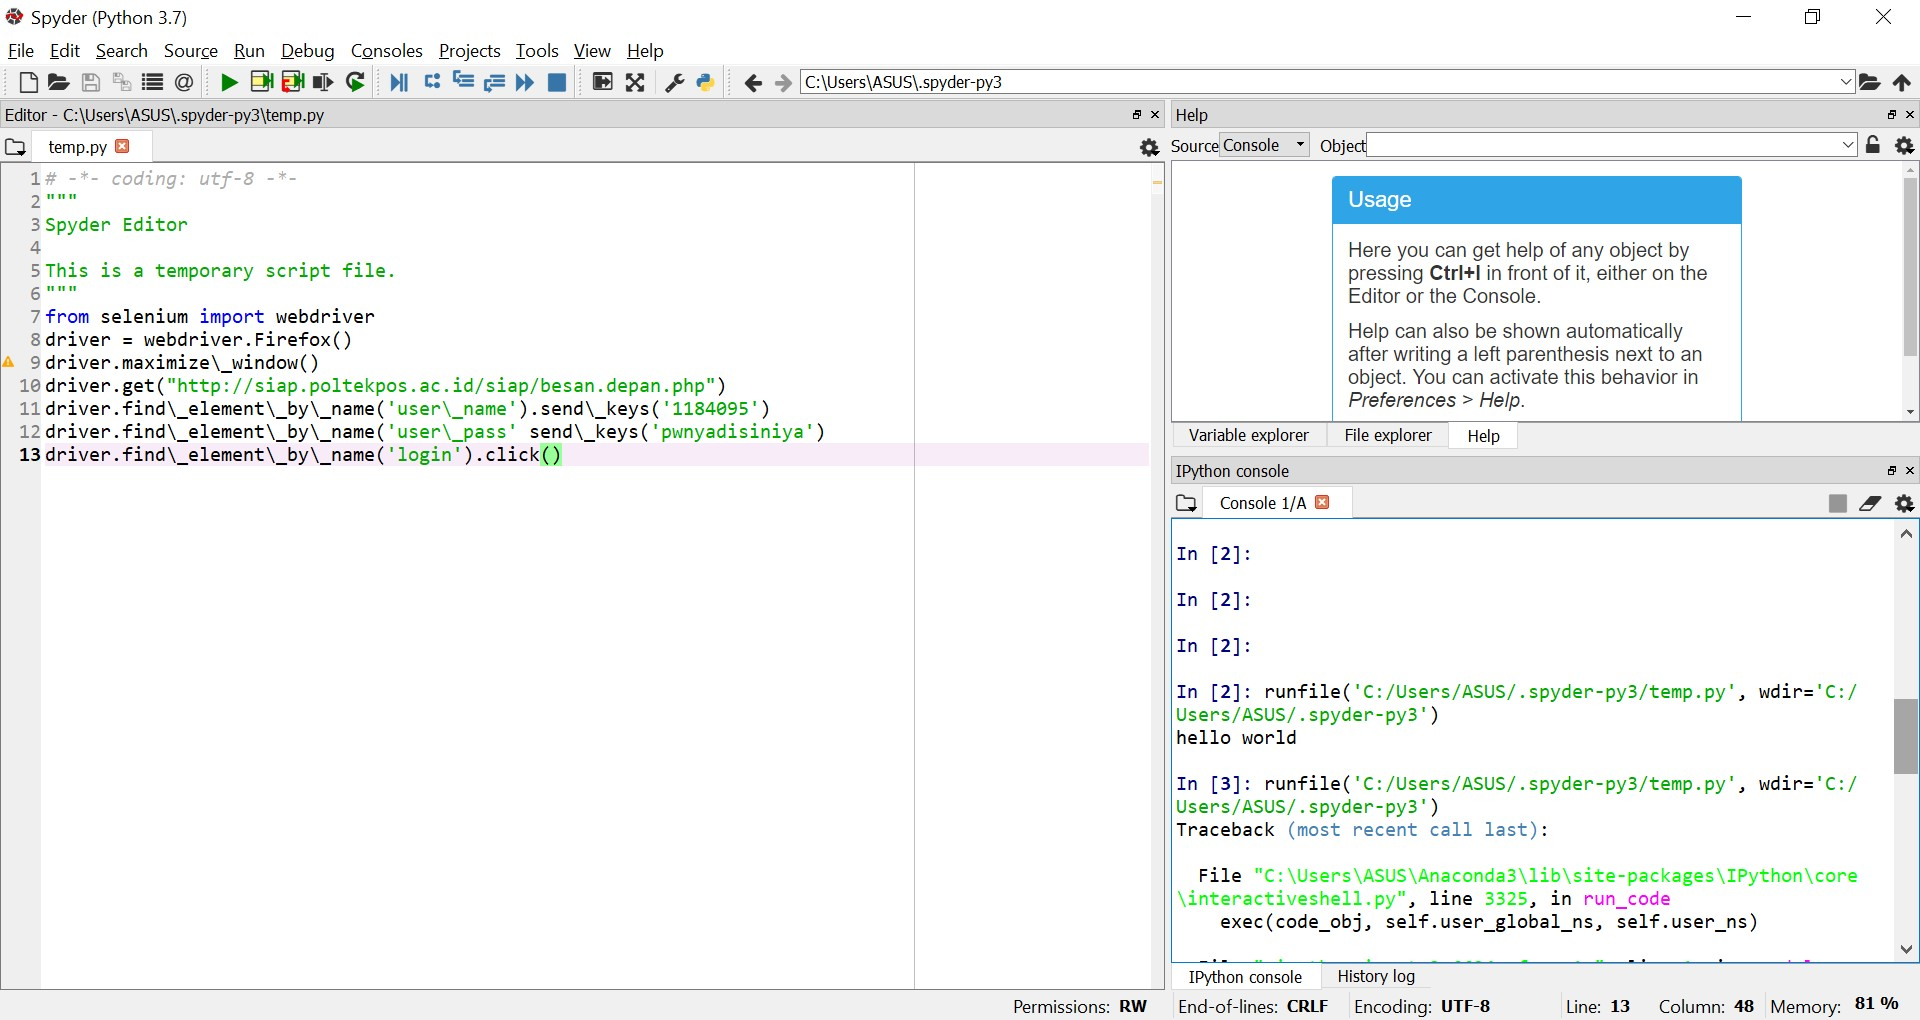
\includegraphics[width = 10cm\textwidth]{selenium.jpg} 
\end{center}

\begin{itemize}
	\item \textit{from selenium import webdriver}, untuk import webdriver
	\item \textit{driver = webdriver.Firefox()},  untuk memilih webdriver firefox
	\item \textit{driver.maximize\_window()},  untuk maximize window browser
	\item \textit{driver.get("http://siap.poltekpos.ac.id/siap/besan.depan.php")}, untuk redirect ke website tujuan
	\item \textit{driver.find\_element\_by\_name('user\_name').send\_keys('1184063')}, untuk mengisi form username, driver akan mencari element dengan nama user\_name
	\item \textit{driver.find\_element\_by\_name('user\_pass').send\_keys('pwnyadisiniya')}, untuk mengisi form password,lalu driver akan mencari element dengan nama pass\_name
	\item \textit{driver.find\_element\_by\_name('login').click()}, untuk klik tombol login, dengan fungsi click()
\end{itemize}

\section{Indentasi}
\subsection{Penjelasan Identasi }
\usepackage{Indentasi merupakan suatu cara perapihan sintaks atau sebagi aturan dalam Bahasa pemrogaman yang akan ditulis. Indentasi digunakan untuk acuan scope pemrograman dan compiler seperti Bahasa pemrograman python. Indentasi ditandai atau berkaitan dengan kurung kurawal ‘’ untuk memulai atau mengakhiri suatu scope permasalahan. Indentasi sering menjadi suatu kebiasaan atau khas dari seorang programmer. Biasanya indentasi dipakai untuk sekedar memudahkan pembacaan kode program, namun dalam Python,Fungsi indentasi sebagai penanda blok kode program.}

\subsection{ jenis jenis error identasi yang didapat}
\usepackage{script pada spyder tidak sesuai posisi, contohnya penulisan script terlalu menjorok atau penulisan yg kurang menjorok ke dalam }

\subsection{Cara membaca eror}
\usepackage{ untuk mengetahui jenis errornya dapat diketahui melalui IndentitionError: expected an idented block. untuk menghindari error ini bisa menggunakan fungsi if memerlukan identasi untuk membedakannya.}

\begin{center}
    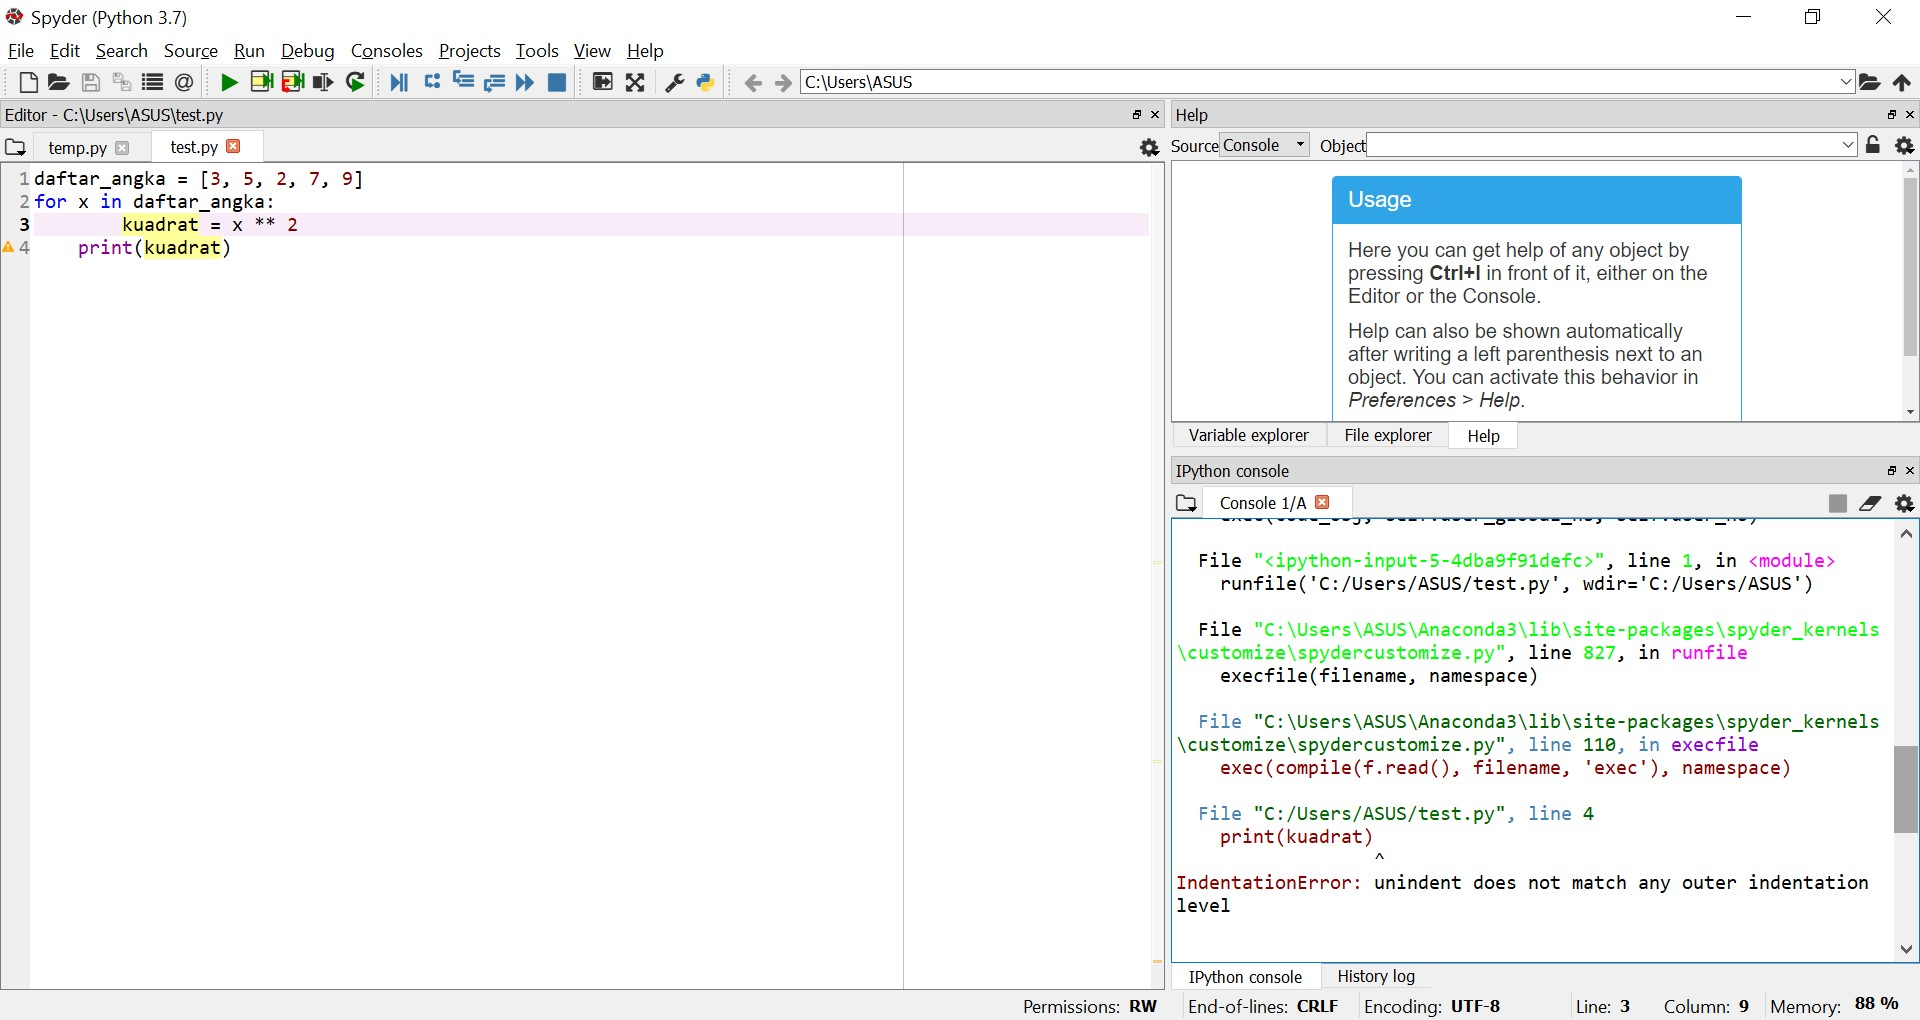
\includegraphics[width = 10 cm]{eror.jpg}
\end{center}

\section{Cara Menangani Eror}
\usepackage{IndentationError: unindent does not match any outer indentation level}

\begin{itemize}
    \item Cara mengatasi eror tersebut, solusinya adalah kita harus mengecek penggunaan tab / spasi dengan konsisten. tapi menurut aturan PEP-8 menyarankan kita menggunakan 4 spasi untuk satu level indentation.
\end{itemize}

\end{document}
